\begin{tikzpicture}[
  delay/.style = {>=Stealth, ->, very thick}]
  \node (client) [] {
\includegraphics[scale = 0.15]{figs/client-pc-logo.png}};
  \node (lms) [below left = 1.8cm and -0.5cm of client] {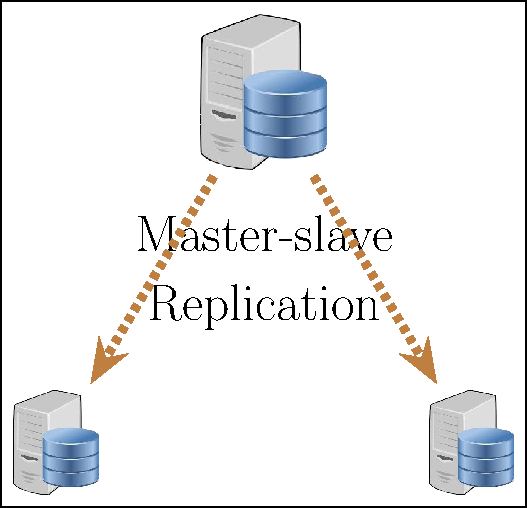
\includegraphics[scale = 0.30]{figs/master-slave.pdf}};
  \node (rms) [below right = 1.8cm and -0.5cm of client] {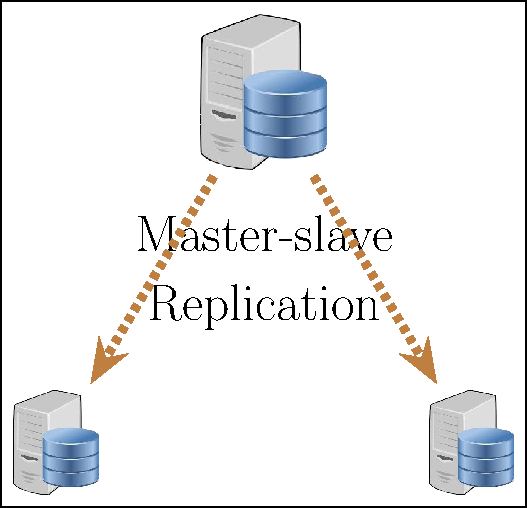
\includegraphics[scale = 0.30]{figs/master-slave.pdf}};

  \uncover<2->{
    % issue delay
    \draw [delay, cyan] (client) to node () [right = -8pt] {issueDelay} ($(lms.north) - (0, 2pt)$);
    \draw [delay, cyan] (client) to ($(rms.south west) + (10pt, 25pt)$);
  }

  \uncover<3->{
    % replication delay
    \draw [delay, teal] ($(rms.north) - (-15pt, 20pt)$) to [bend left] 
    node () [above, sloped] {replDelay} ($(rms.south east) - (15pt, -25pt)$);
  }

  \uncover<4->{
    % 2pc delay
    \draw [delay, blue] ($(lms.north) - (-15pt, 20pt)$) to node () [above] {2pcDelay} ($(rms.north) - (15pt, 20pt)$);
  }
\end{tikzpicture}